\documentclass{beamer}

\usepackage[utf8]{inputenc}
\usepackage{default}
\usepackage{amsmath}
\usepackage{upgreek}
\usepackage{booktabs}
\usepackage{verbatim}

\title{Konstruksjon av høydimensjonale nevralt nettverk-potensialer for molekylærdynamikk}
\author{John-Anders Stende}
\institute{
  Fysisk institutt \\
  Universitetet i Oslo
}
\date{Masterpresentasjon, oktober 2017}
\subject{Computational physics}

\AtBeginSection[]
{
  \begin{frame}
    \frametitle{Table of Contents}
    \tableofcontents[currentsection]
  \end{frame}
}

\begin{document}

\frame{\titlepage}

\begin{frame}

\tableofcontents

\end{frame}


\section{Molekylærdynamikk}


\begin{frame}

\begin{block}{Hva er molekylærdynamikk?}
  \begin{itemize}
  \item Numerisk metode for å simulere atomers og molekylers bevegelser i gasser, væsker og faste stoffer.
  \item Virtuelt eksperiment.
  \end{itemize}
\end{block}

\end{frame}


\begin{frame}

\begin{block}{Dynamikk}
  \begin{itemize}
  \item Partiklenes interaksjoner styrer dynamikken.
  \item Interaksjonene bestemmes av et kraftfelt $\mathbf{F}$:
    \begin{equation*}
    \mathbf{F} = -\nabla V(\mathbf{r})
    \end{equation*}
  \item Potensiell energiflate / potensial):
    \begin{equation*}
      V(\mathbf{r}), \quad \mathbf{r} = (\mathbf{r}_1, \mathbf{r}_2, \cdots, \mathbf{r}_N)
    \end{equation*}
  \item $V(\mathbf{r})$ inneholder fysikken. 
  \end{itemize}
\end{block}

\end{frame}


\begin{frame}

\begin{columns}[T] % contents are top vertically aligned
  \begin{column}[T]{0.5\linewidth} % each column can also be its own environment
    \begin{block}{Ab inito molekylærdynamikk}
    Løse Schrödinger-likningen ved hvert tidssteg.
    \end{block}
  \end{column}
  \begin{column}[T]{0.5\linewidth} % alternative top-align that's better for graphics
    \begin{block}{Klassisk molekylærdynamikk}
    Bruke en predefinert analytisk funksjon.
    \end{block}
  \end{column}
\end{columns}

\end{frame}


\begin{frame}

\begin{block}{Klassisk potensial}
  \begin{equation*}
  V(\mathbf{r}) \approx \sum_i^N V_1(\mathbf{r}_i) + \sum_{i,j}^N V_2(\mathbf{r}_i, \mathbf{r}_j) + 
  \sum_{i,j,k}^N V_3(\mathbf{r}_i, \mathbf{r}_j, \mathbf{r}_k) + \dots
  \end{equation*}
\end{block}

\begin{enumerate}
 \item Hvor mange ledd bør tas med?
 \item Hvordan bør leddene se ut?
\end{enumerate}

Eksperiementer / kvantemekanikk

\end{frame}


\begin{frame}

\begin{block}{Empirisk potensial:}
 \begin{enumerate}
  \item Starte med en funksjonsform med noen parametre.
  \item Bestemme parametre fra eksperimentelle data.
 \end{enumerate}
\end{block}

\begin{block}{Kvantemekanisk potensial:}
 \begin{enumerate}
  \item Produsere kvantemekaniske data. 
  \item Tilpasse en generell funksjonsform til datasettet.
 \end{enumerate}
 
 \begin{itemize}
  \item Fordeler: Ab inito nøyaktighet, ingen bias, overførbart.
  \item Ulemper: Rent matematisk uttrykk, all relevant data må inkluderes. 
 \end{itemize}
\end{block}

\end{frame}


\begin{frame}
 
\begin{block}{Interpolere datasett}
 \begin{itemize}
  \item Spliner
  \item Minste kvadraters metode
  \item Kunstige nevrale nettverk
 \end{itemize}
\end{block}
 
\end{frame}


\section{Nevrale nettverk}


\begin{frame}

\begin{block}{Kunstige nevrale nettverk}
 \begin{itemize}
  \item Maskinlæringsalgortime.  
  \item Etterlikner biologiske nevrale nettverk.
  \item Kunstige nevroner sender signaler i form av matematiske funksjoner. 
 \end{itemize}
\end{block}

\end{frame}


\begin{frame}
 
\centering
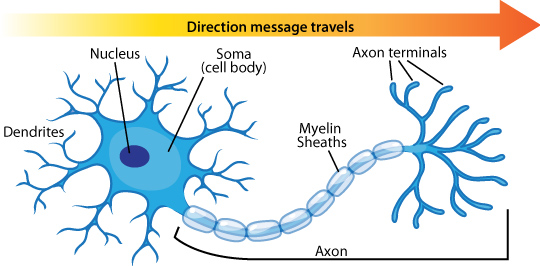
\includegraphics[width=0.8\linewidth]{../Figures/Theory/neuron_anatomy.jpg} 

\end{frame}


\begin{frame}

\centering
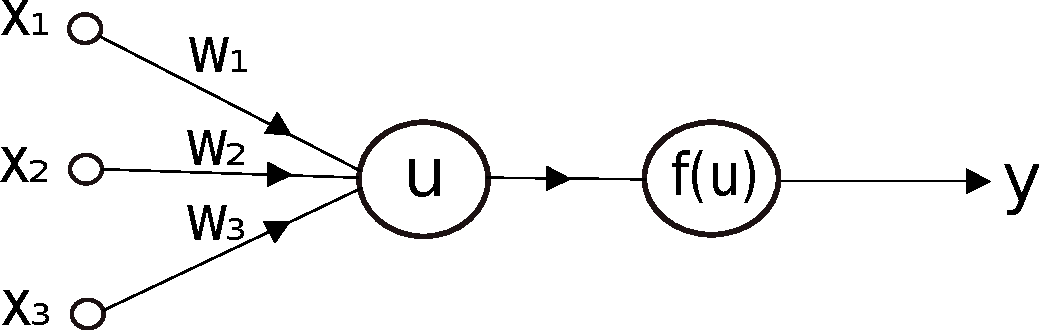
\includegraphics[width=0.8\linewidth]{../Figures/Theory/neuron.pdf} 

\begin{equation*}
 y = f\left(\sum_{i=1}^n w_ix_i + b_i\right) = f(u)
\end{equation*}

\begin{itemize}
 \item $x_i$: Inputsignaler.
 \item $w_i$: Vekter - forsterkning/forminksning.  
 \item $u$: Sum - signalmiksing i soma.
 \item $f(u)$: Akteriveringsfunksjon - aksjonspotensial.
\end{itemize}

\end{frame}


\begin{frame}
 
\centering
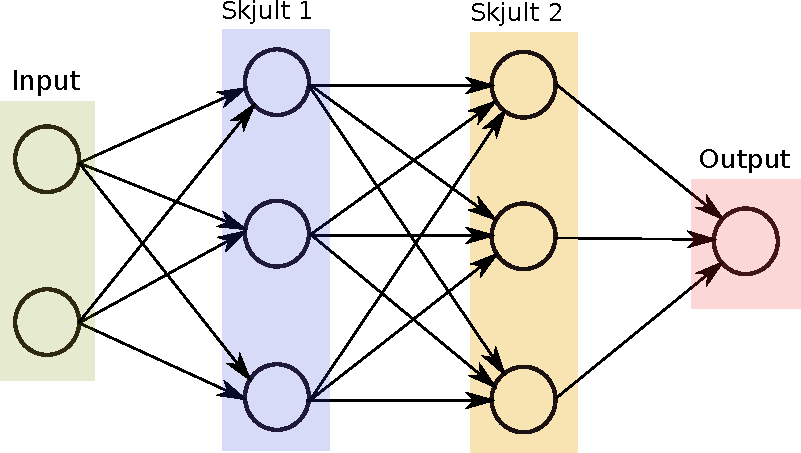
\includegraphics[width=0.8\linewidth]{../Figures/Presentation/networkGeneral.pdf}

\begin{block}{Fully-connected feed-forward nettverk.}
 \begin{itemize}
  \item Hvert nevron i et lag er koblet til alle nevroner i neste lag. 
  \item Informasjon propagares kun fremover fra input til output.
 \end{itemize}
\end{block}

\end{frame}


\begin{frame}{Detaljert beskrivelse}
 
\centering
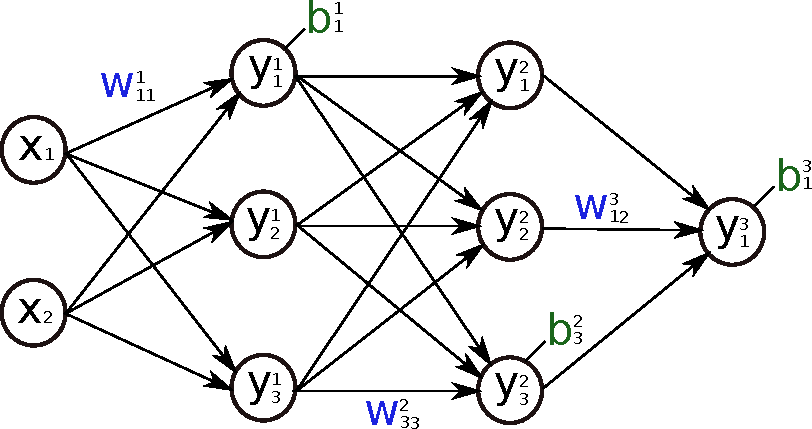
\includegraphics[width=0.8\linewidth]{../Figures/Theory/networkWithNotationAltered.pdf}

\begin{itemize}
 \item Hver forbindelse/pil har en vekt $w$. 
 \item Hver node har en bias $b$.
 \item Inneholder 25 parametre $\{w,b\}$
\end{itemize}

\end{frame}


\begin{frame}{Analytisk uttrykk}

\begin{align*}
  y_1^3 &= f_3\left[\sum_{j=1}^3 w_{1j}^3 f_2\left(\sum_{k=1}^3 w_{jk}^2 f_1\left(\sum_{m=1}^2 w_{km}^1 x_m + b_k^1\right) + b_j^2\right)
  + b_1^3\right] \\
  &= f_3(x_1, x_2)
\end{align*}
\begin{itemize}
 \item Mapping: $(x_1, x_2) \in \mathbb{R}^2  \rightarrow y_1^3 \in \mathbb{R}$. 
 \item Ved å justere de 25 parameterne får uttrykket stor fleksibilitet. 
 \item Dimensjonene til nettet (inputs og outputs) må stemme overens med funksjonen som skal tilpasses.
 \item Et nettverk med ett skjult lag kan approksimere enhver kontinuerlig funksjon. 
\end{itemize}


\end{frame}


\begin{comment}\begin{frame}{Aktiveringsfunksjoner}

\begin{block}{Restriksjoner}
 \begin{itemize}
  \item Ikke-konstant
  \item Begrenset
  \item Monotont økende
  \item Kontinuerlig
 \end{itemize}

\end{block}

\begin{columns}[T] % contents are top vertically aligned

 \begin{column}[T]{0.5\linewidth} % each column can also be its own environment
  The sigmoid
  \begin{equation*}
  f(x) = \frac{1}{1 + e^{-x}}
  \label{sigmoidActivationFunction}
  \end{equation*}
  og hyperbolsk tangens
  \begin{equation*}
  f(x) = \tanh(x)
  \label{tanhActivationFunction}
  \end{equation*}
 \end{column}
 
 \begin{column}[T]{0.5\linewidth} % alternative top-align that's better for graphics
  \centering
  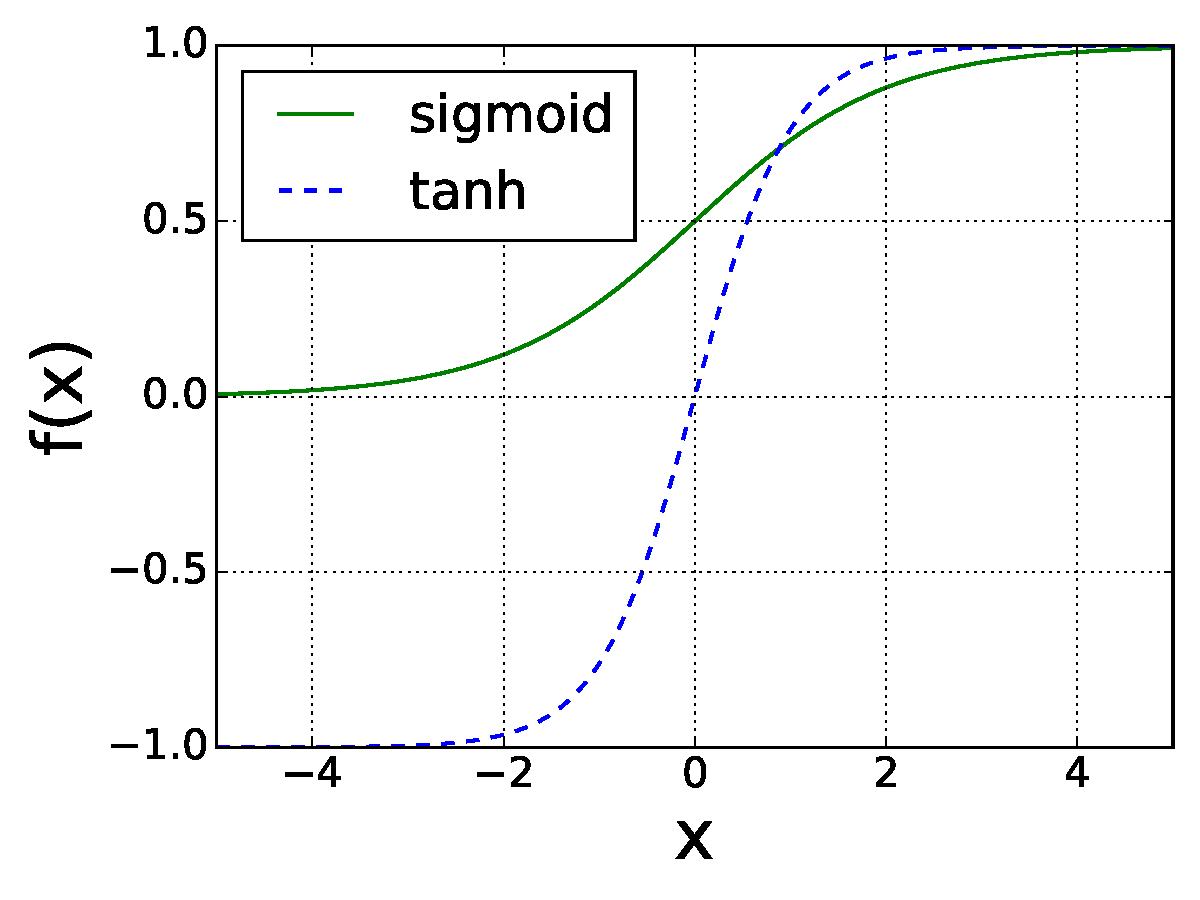
\includegraphics[width=\linewidth]{../Figures/Theory/activationFunctionsAltered.pdf}
 \end{column}
 
\end{columns}
  
\end{frame}\end{comment}


\begin{frame}
 
\centering
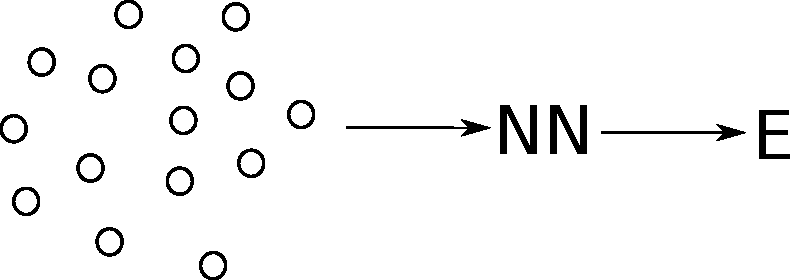
\includegraphics[width=0.8\linewidth]{../Figures/Presentation/interpolation.pdf}
\begin{block}{Regresjon med nevralt nettverk}
 \begin{itemize}
  \item Mål: Interpolere datasett av konfigurasjoner $X$ og energier $Y$ slik at
        $\mathrm{NN}: \mathrm{X} \in \mathbb{R}^n \rightarrow \mathrm{Y} \in \mathbb{R}$.
  \item Referansenergiene $Y$ regnes ut kvantemekanisk. 
  \item Trening: Iterativt justere parameterne slik at nettets output matcher referanseenergiene.
  \item Én enkelt konfigurasjon kalles et \textit{treningseksempel}. 
 \end{itemize}
\end{block}

\end{frame}


\begin{frame}
 
\begin{block}{Feilen til nettet defineres ved en cost-funksjon:} 
 Gjennomsnittlig kvadratisk feil:
 \begin{equation*}
 \Gamma = \frac{1}{2N}\sum_{i=1}^N (Y_i - y_i)^2
 \end{equation*}
\end{block}

\begin{block}{Cost-funksjonen minimieres med gradient descent:}
 \begin{equation*}
  \boldsymbol{\uptheta}_{k+1} = \boldsymbol{\uptheta}_{k} - \gamma \nabla_{\boldsymbol{\uptheta}_k} \Gamma(\boldsymbol{\uptheta})
 \end{equation*}
 \begin{itemize}
  \item $\boldsymbol{\uptheta}_{k}$: Vektor av parametre ved iterasjon $k$. 
  \item $\gamma$: Steglengde/læringsrate. 
 \end{itemize}
\end{block}

\end{frame}


\begin{frame}{Hvordan finne gradienten av et nevralt nettverk?}

\begin{equation*}
  y_1^3 = f_3\left[\sum_{j=1}^3 w_{1j}^3 f_2\left(\sum_{k=1}^3 w_{jk}^2 f_1\left(\sum_{m=1}^2 w_{km}^1 x_m + b_k^1\right) + b_j^2\right)
  + b_1^3\right]
\end{equation*}

\begin{block}{Backpropagation}
 \begin{itemize} 
  \item Verdien av cost-funksjonen (feilen) propagares \textit{bakover} fra output til input.
  \item Alle deriverte innhentes ved å propagere feilen én gang. 
  \item En anvendelse av kjerneregelen. 
 \end{itemize}
\end{block}
 
\end{frame}


\section{Nevralt nettverk-potensial}


\begin{frame}
 
\begin{block}{Hvor mange nettverk?}
 \begin{itemize}
  \item Ett nettverk: Uhåndterlig størrelse. 
  \item Atomære nettverk,
   \begin{equation*}
    E = \sum_{i=1}^N E_i
   \end{equation*}
   \item Behler-Parrinello: Hver atomenergi $E_i$ avhenger kun av naboatomer innenfor en cutoff-radius $r_c$. 
 \end{itemize}
\end{block}

\end{frame}


\begin{frame}

\begin{block}{Høydimensjonalt potensial - utfordringer}
 \begin{enumerate} 
  \item Varierende antall naboer. 
  \item Translasjonell og rotasjonell invarians. 
  \item Rekkefølgen på naboer. 
 \end{enumerate}
\end{block}

\begin{block}{Behler-Parrinello-metoden: Symmetrifunksjoner}
 \begin{enumerate}
  \item Et sett av såkalte symmetrifunksjoner transformerer de kartesiske koordinatene til alle naboer 
  til en vektor av symmetriverdier.
  \item Symmetrifunksjonene er atomsentrerte. 
  \item Symmetrifunksjonene er definert som summer over naboer. 
 \end{enumerate}
\end{block}

\end{frame}


\begin{frame}{Behler-Parrinello eksempel}

\begin{itemize}
 \item Symmetrifunksjone beskriver hvert atoms kjemiske omgivelser. 
 \item Hvert atom har både et eget nettverk og et eget sett av symmetrifunksjoner.  
 \item Alle atomer av samme kjemiske element har identiske nettverk og symmetrifunksjonssett. 
\end{itemize}

\begin{columns}[c] % contents are top vertically aligned
  \begin{column}[c]{0.35\linewidth} % each column can also be its own environment
   \centering
   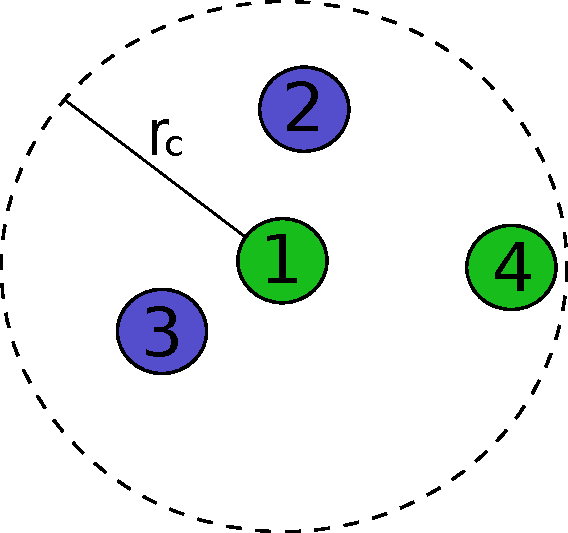
\includegraphics[width=\linewidth]{../Figures/Presentation/cutoffSphere.pdf}
  \end{column}
  \begin{column}[c]{0.65\linewidth} % alternative top-align that's better for graphics
   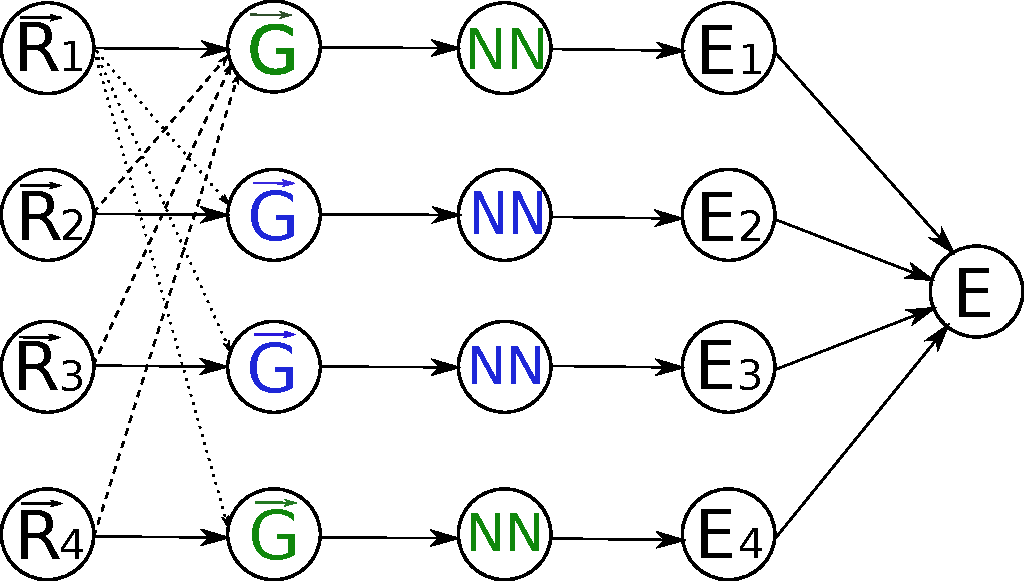
\includegraphics[width=\linewidth]{../Figures/Presentation/BehlerParrinello.pdf}
  \end{column}
\end{columns}

\end{frame}


\begin{frame}

\begin{block}{Cutoff-funksjon}
 Monotonisk minkende del av en cosinus-funksjon. 
 \begin{equation*}
  f_c(r_{ij}) = 
  \begin{cases}
   0.5 \!\left[\cos\left(\pi r_{ij}/r_c\right) + 1 \right], & r_{ij} \leq r_c \\
   0, & r_{ij} > r_c
  \end{cases}
 \end{equation*}
 \centering
 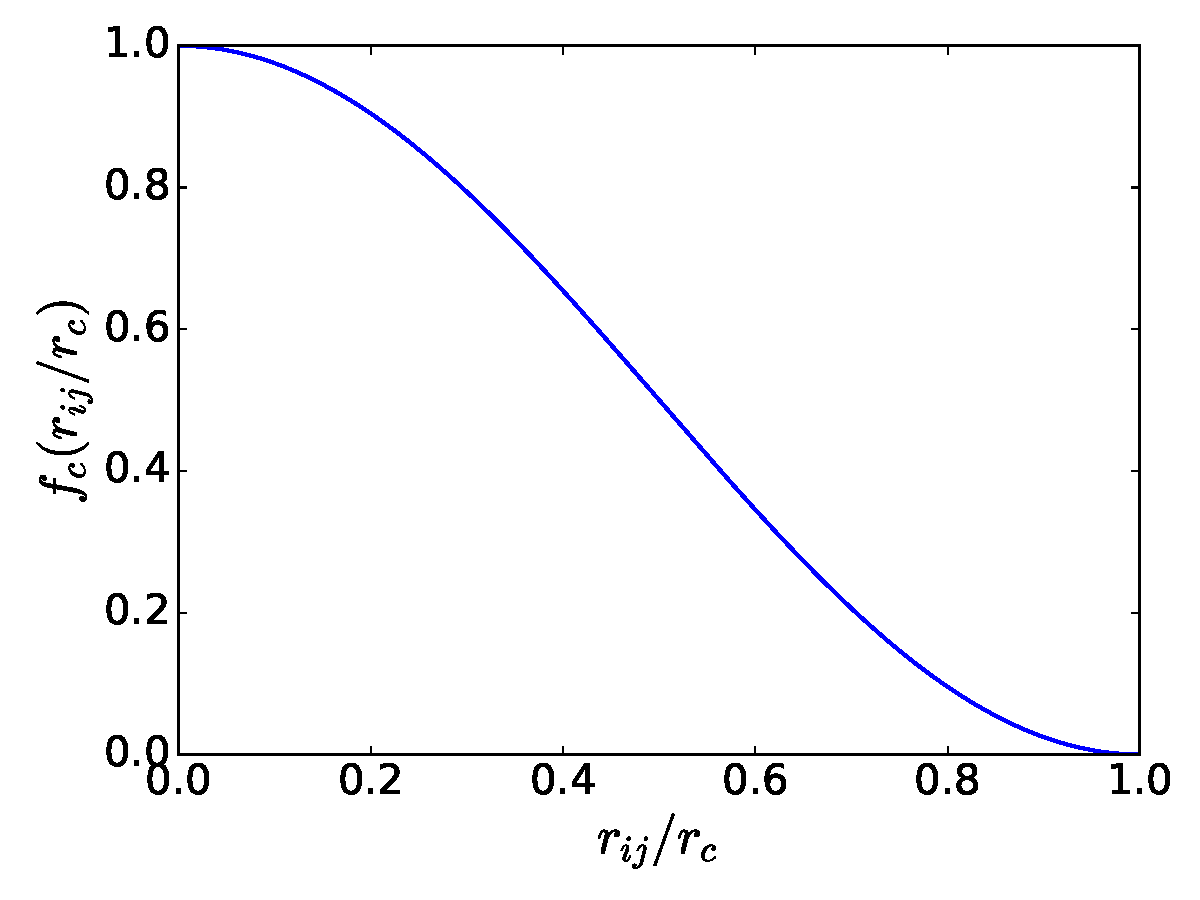
\includegraphics[width=0.7\linewidth]{../Figures/Presentation/cutoffFunction.pdf}
\end{block}

\end{frame}


\begin{frame}{Radiell symmetrifunksjon}

\begin{equation*}
 G_i^\mathrm{rad} = \sum_{j=1}^N \exp[-\eta(r_{ij}-r_s)^2] \,f_c(r_{ij})
\end{equation*}
\newline
\centering
For ett enkelt naboatom
\begin{columns} % contents are top vertically aligned
  \begin{column}{0.5\linewidth} % each column can also be its own environment
   \centering
   $r_s = 0$
   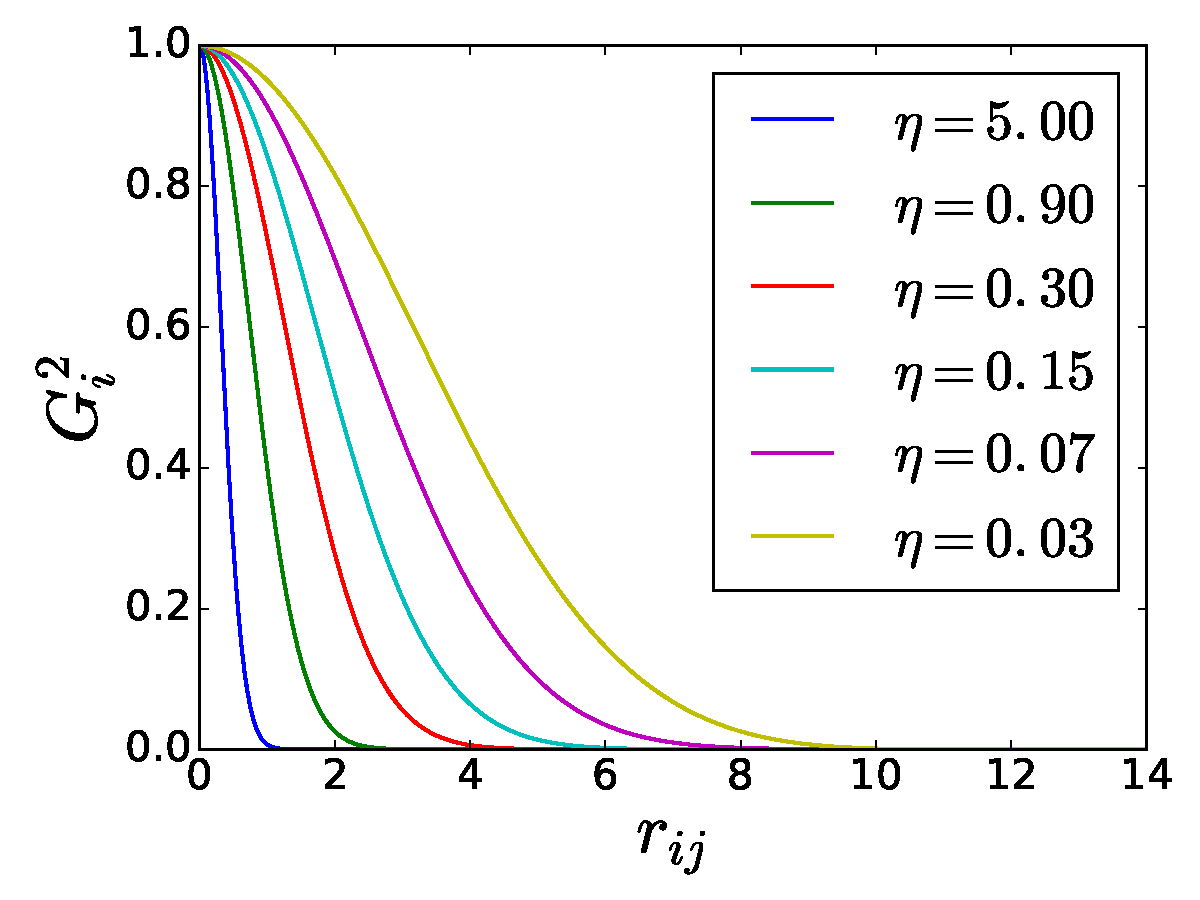
\includegraphics[width=\linewidth]{../Figures/Presentation/G2_1.pdf}
  \end{column}
  \begin{column}{0.5\linewidth} % alternative top-align that's better for graphics
   \centering
   $\eta = 3.0$
   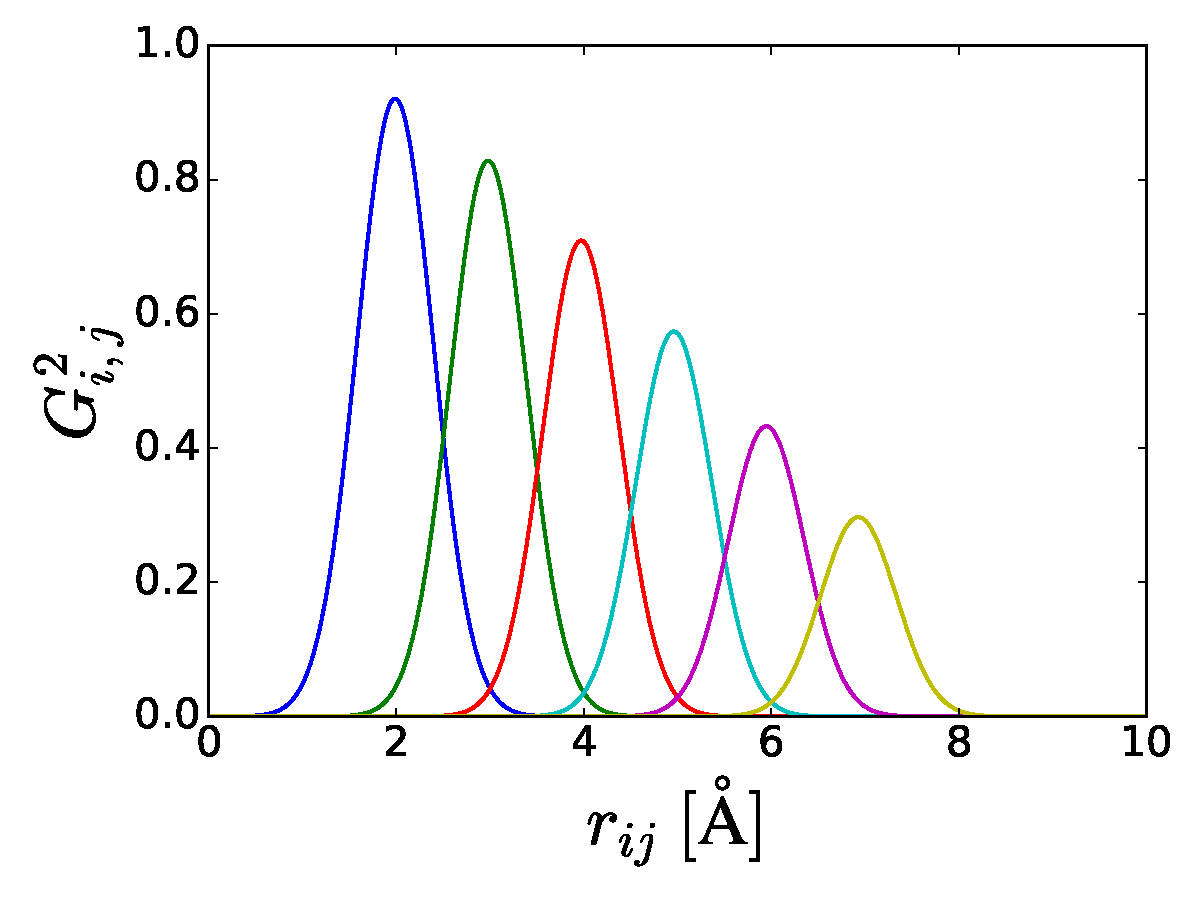
\includegraphics[width=\linewidth]{../Figures/Presentation/G2_2.pdf}
  \end{column}
\end{columns}

\end{frame}


\begin{frame}{Angulær symmetrifunksjon}

\begin{equation*}
  G_i^\mathrm{ang} = 2^{1-\zeta}\sum_{j\neq i}\sum_{k>j} \Big[(1 + \lambda \cos\theta_{jik})^\zeta \,
 \exp[-\eta (r_{ij}^2 + r_{ik}^2)] \,
 &f_c(r_{ij}) f_c(r_{ik})\Big]
\end{equation*}

\centering
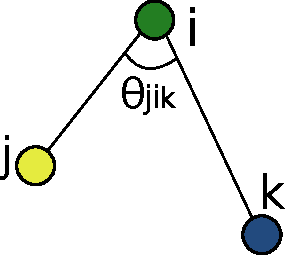
\includegraphics[width=0.17\linewidth]{../Figures/Presentation/triplet.pdf}

\begin{columns} % contents are top vertically aligned
  \begin{column}{0.5\linewidth} % each column can also be its own environment
   \centering
   $\lambda = +1$
   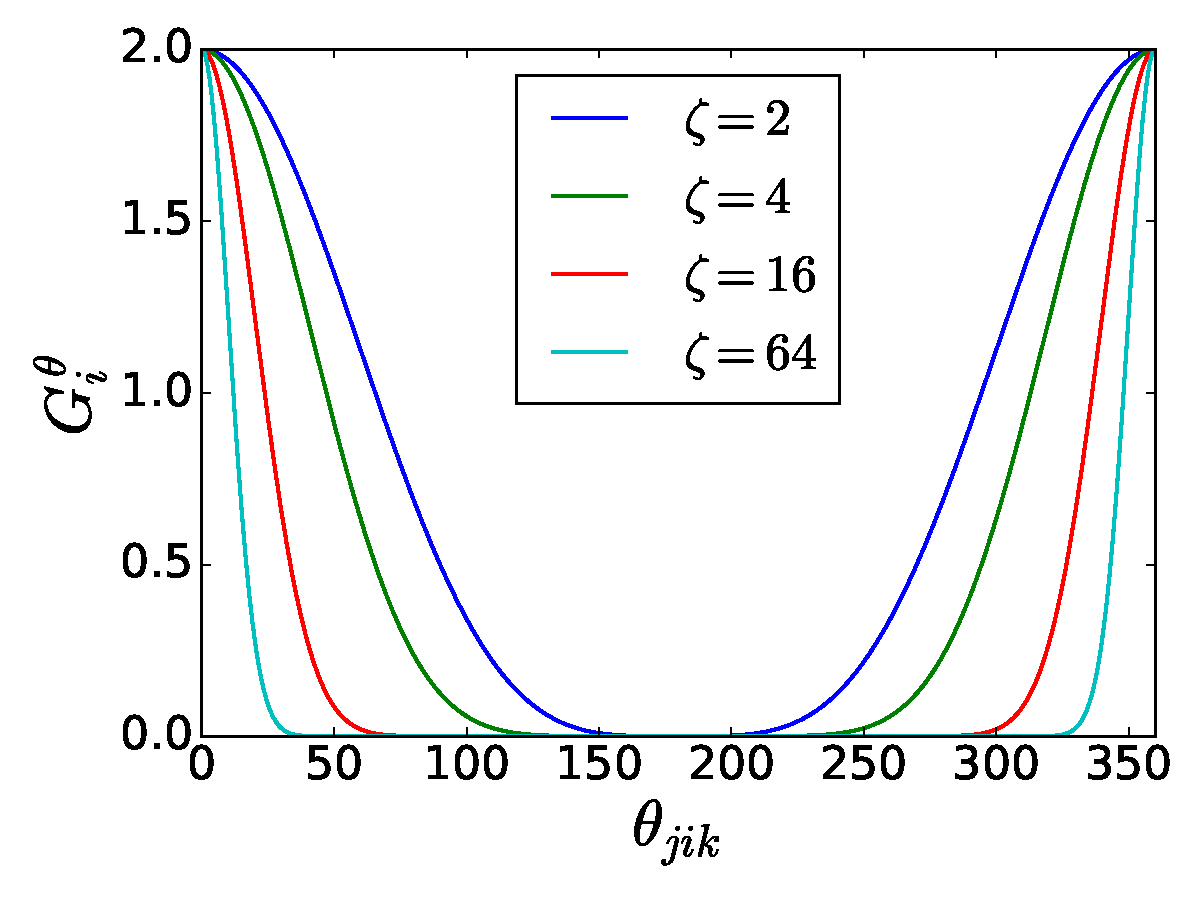
\includegraphics[width=\linewidth]{../Figures/Presentation/G4G5angular1.pdf}
  \end{column}
  \begin{column}{0.5\linewidth} % alternative top-align that's better for graphics
   \centering
   $\lambda = -1$
   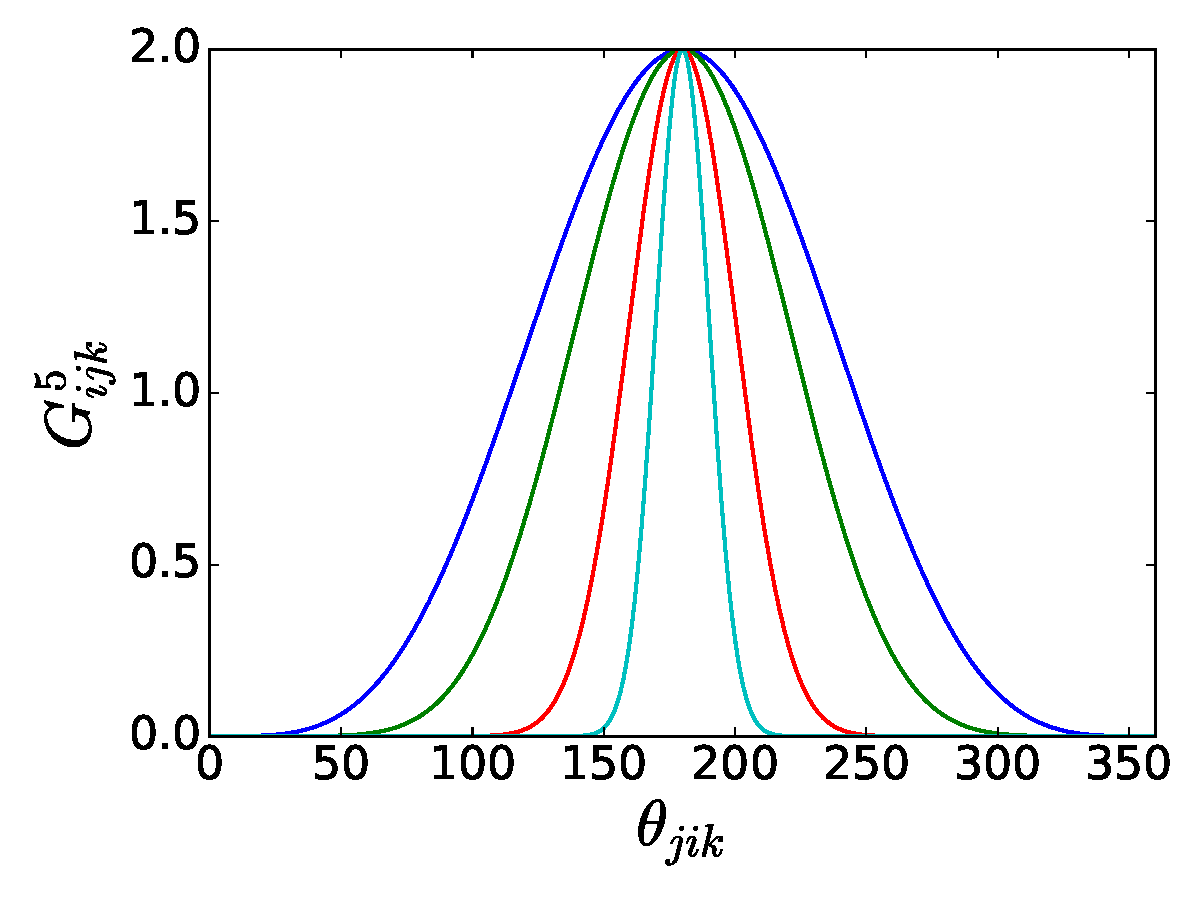
\includegraphics[width=\linewidth]{../Figures/Presentation/G4G5angular2.pdf}
  \end{column}
\end{columns}

\end{frame}


\begin{frame}

\begin{block}{Krefter for et grunnstoff}
 \begin{equation*}
  \mathbf{F}_i = -\nabla_i E
 \end{equation*}

 \begin{equation*}
  F_{i,x} = -\frac{\partial E}{\partial x_i} =
  -\sum_{j=1}^{N_i+1}\frac{\partial E_j}{\partial x_i} = 
  -\sum_{j=1}^{N_i+1}\sum_{s=1}^M\frac{\partial E_j}{\partial G_s}\frac{\partial G_s}{\partial x_i}
 \end{equation*}
 \begin{equation*}
  E_j = \mathrm{NN}[\mathbf{G}(\mathbf{r}_{jk})]
 \end{equation*}
\end{block}

\end{frame}


\section{NNP for Si}


\begin{frame}{Simuleringspakker}

\begin{block}{LAMMPS}
 \begin{itemize}
  \item Pakke for klassisk molekylærdynamikk utviklet ved Sandia National Laboratories. 
  \item Kjøres ved inputscripts med egen syntaks. 
  \item Vi har utvidet med samplingsalgoritme og nevralt nettverk-potensial.
 \end{itemize}
\end{block}

\begin{block}{TensorFlow}
 \begin{itemize}
  \item Maskinlæringspakke utviklet av Google. 
  \item Vi har brukt TensorFlow Python API til å utvikle en modell for regresjon med nevrale nettverk. 
 \end{itemize}
\end{block}

\end{frame}


\begin{frame}

\begin{block}{Konstruksjon av et nevralt nettverk-potensial (NNP)}
 \begin{enumerate}
  \item Generere treningsdata som er relevant for applikasjonen av NNP. 
  \item Trene et nevralt nettverk for å tilpasse en funksjon til dataene. 
  \item Bruke det trente nettverket som et analytisk potensial i molekylærdynamikksimuleringer. 
 \end{enumerate}
\end{block}

\end{frame}


\begin{frame}
 
\centering
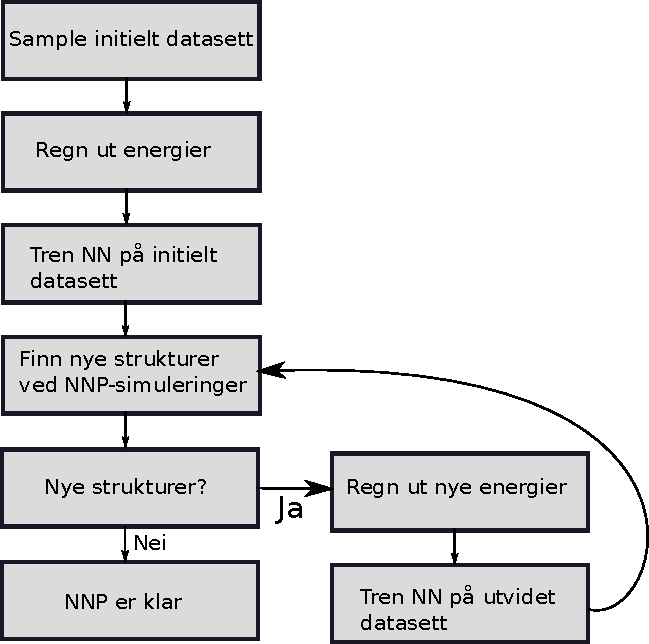
\includegraphics[width=0.7\linewidth]{../Figures/Presentation/iterativeSampling.pdf} 

\end{frame}


\begin{frame}

\begin{block}{Initiell sampling}
 \begin{itemize}
  \item Stillinger-Weber. 
  \item $T \in [0,500]$ K. 
  \item Konfigurasjoner og energies samples med samplingsalgoritme.  
 \end{itemize}
\end{block}

\end{frame}


\begin{frame}

\begin{columns} % contents are top vertically aligned
  \begin{column}{0.5\linewidth} % each column can also be its own environment
   \centering
   Radielle
   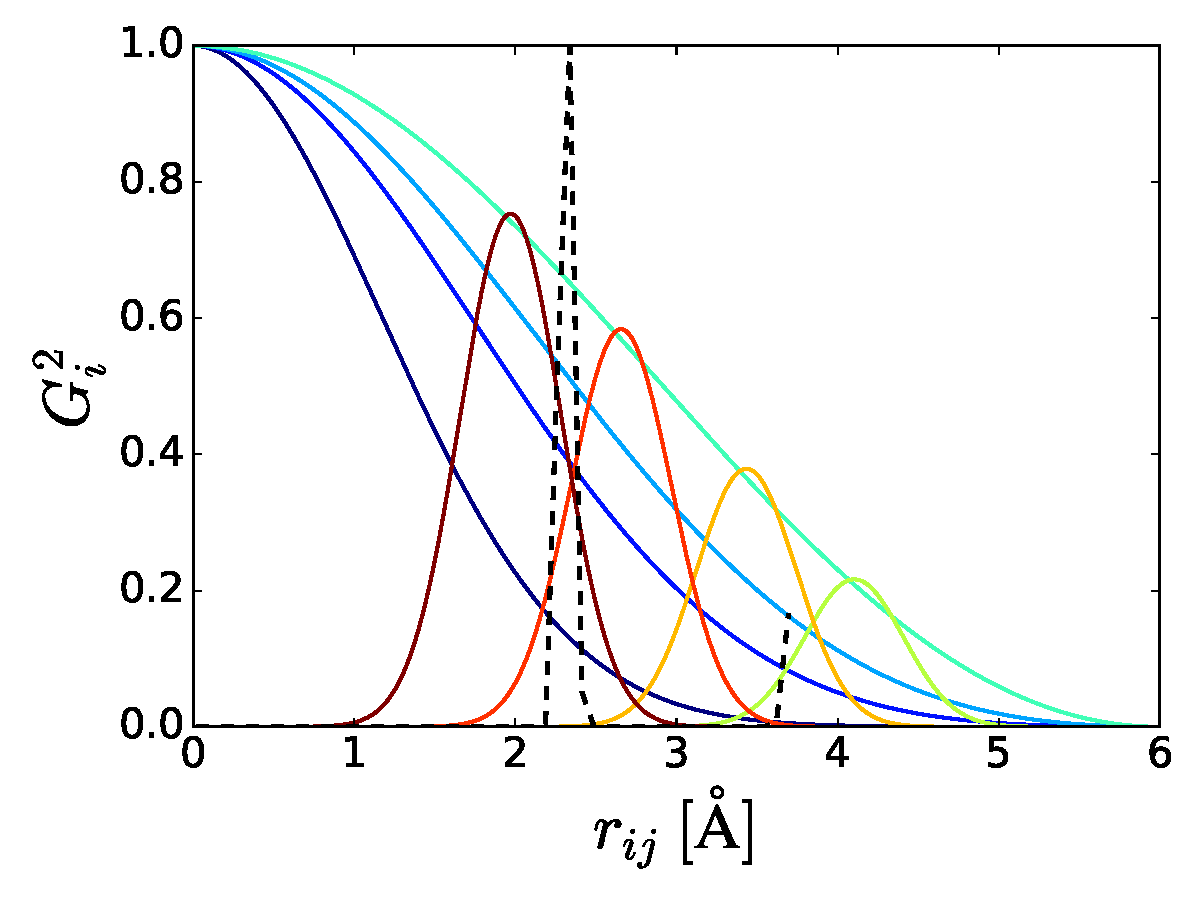
\includegraphics[width=\linewidth]{../Figures/Presentation/SiInitialSymmG2.pdf}
  \end{column}
  \begin{column}{0.5\linewidth} % alternative top-align that's better for graphics
   \centering
   Angulære
   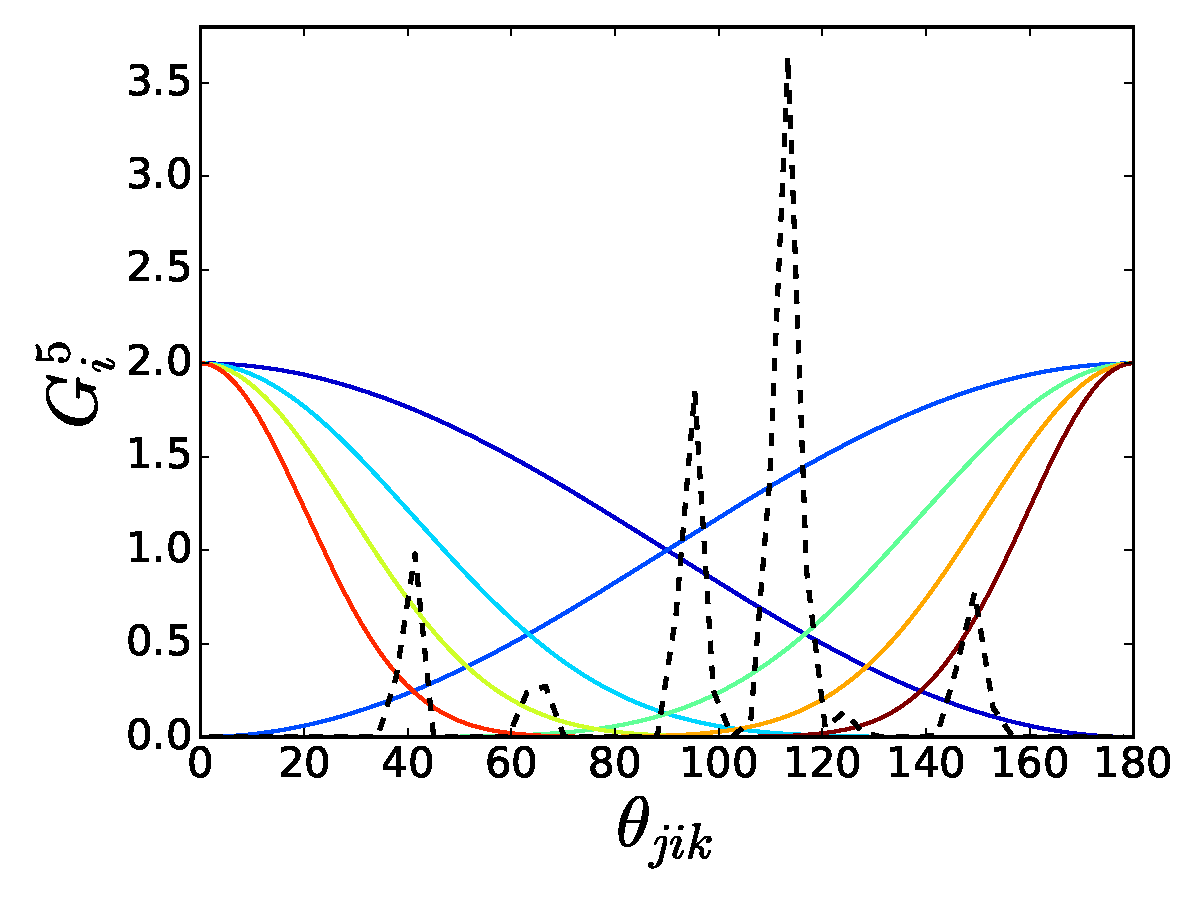
\includegraphics[width=\linewidth]{../Figures/Presentation/SiInitialSymmG5.pdf}
  \end{column}
\end{columns}
 
\end{frame}


\begin{frame}

\begin{block}{Ekstrapolasjon}
 Lagre max og min for hver symmetryfunksjon. 
\end{block}

\begin{block}{Interpolasjon - multiple-NN-metoden}
 \centering
 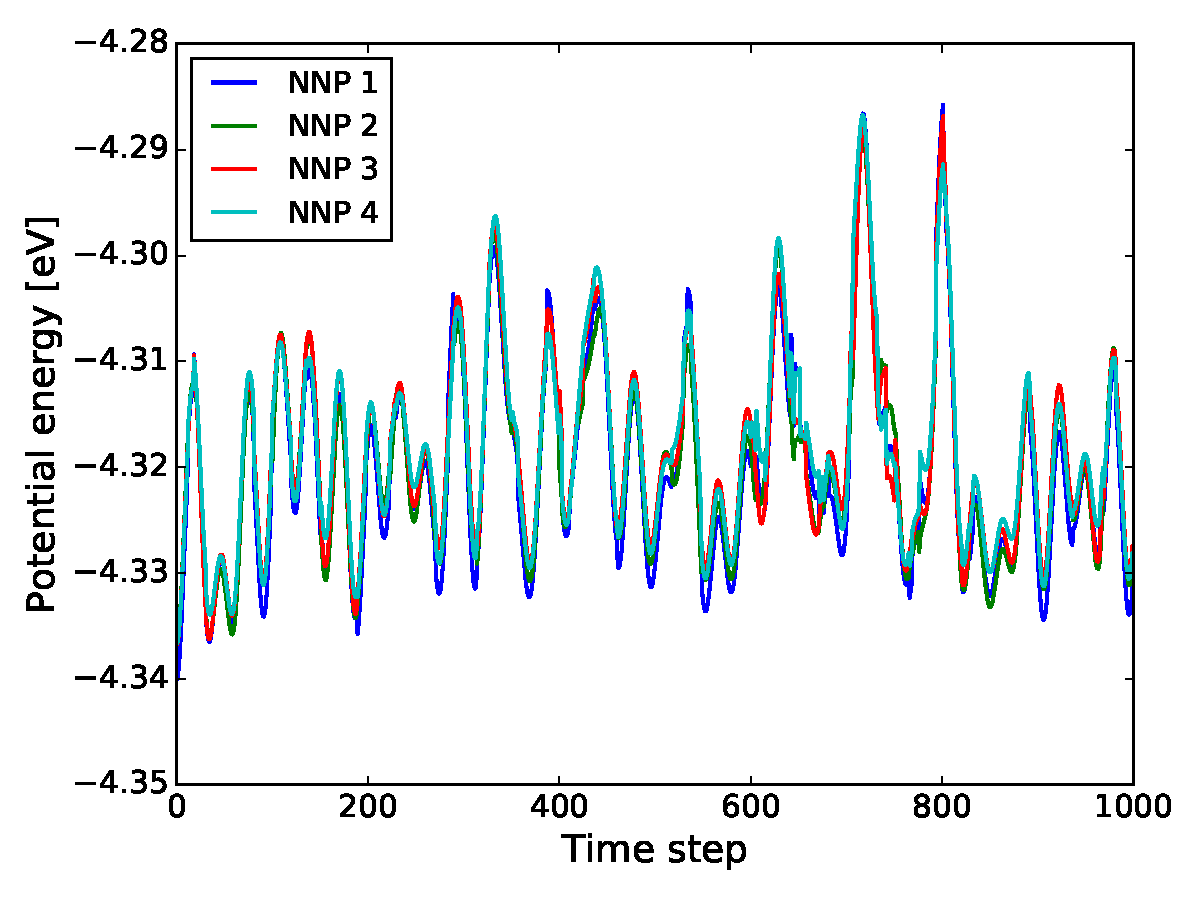
\includegraphics[width = 0.7\linewidth]{../Figures/Results/multipleNNP.pdf}
\end{block}

\end{frame}


\begin{frame}{Gridsøk}
 
\renewcommand{\arraystretch}{0.9}
\begin{table} 
\centering
  \begin{tabular*}{10cm}{l @{\extracolsep{\fill}} llll}
    \toprule
    Layers & Nodes & RMSE & Epoch & Time \\ 
    \hline
    $L=1$ & 4  & 4.445 & 37035 & 575 \\
	  & 8  & 2.250 & 37305 & 570 \\
	  & 12 & 2.303 & 37980 & 622 \\
	  & 16 & 2.201 & 39780 & 630 \\
	  & 20 & 1.860 & 36180 & 617 \\ 
	  & 24 & 1.928 & 37305 & 621 \\
	  & 28 & 2.407 & 39375 & 697 \\
	  & 32 & 2.214 & 38700 & 672 \\
    $L=2$ & 4  & 2.947 & 39960 & 750 \\
	  & 8  & 1.933 & 36180 & 671 \\
	  & 12 & 1.450 & 37350 & 766 \\
	  & 16 & 1.791 & 32265 & 633 \\
	  & 20 & 1.492 & 24840 & 546 \\
	  & 24 & 2.118 & 37620 & 819 \\
	  & 28 & 1.455 & 37350 & 895 \\
	  & 32 & 2.008 & 14895 & 344 \\
    \bottomrule
    \end{tabular*} 
\end{table}

\end{frame}


\begin{frame}
 
\begin{block}{Tilpasse endelig treningssett}
 Velger nettet med lavest RMSE etter 40000 epoker. RMSE: 0.864 meV.
\end{block}

\begin{block}{RMSE krefter}
 \centering
 RMSE: 41.2 meV
 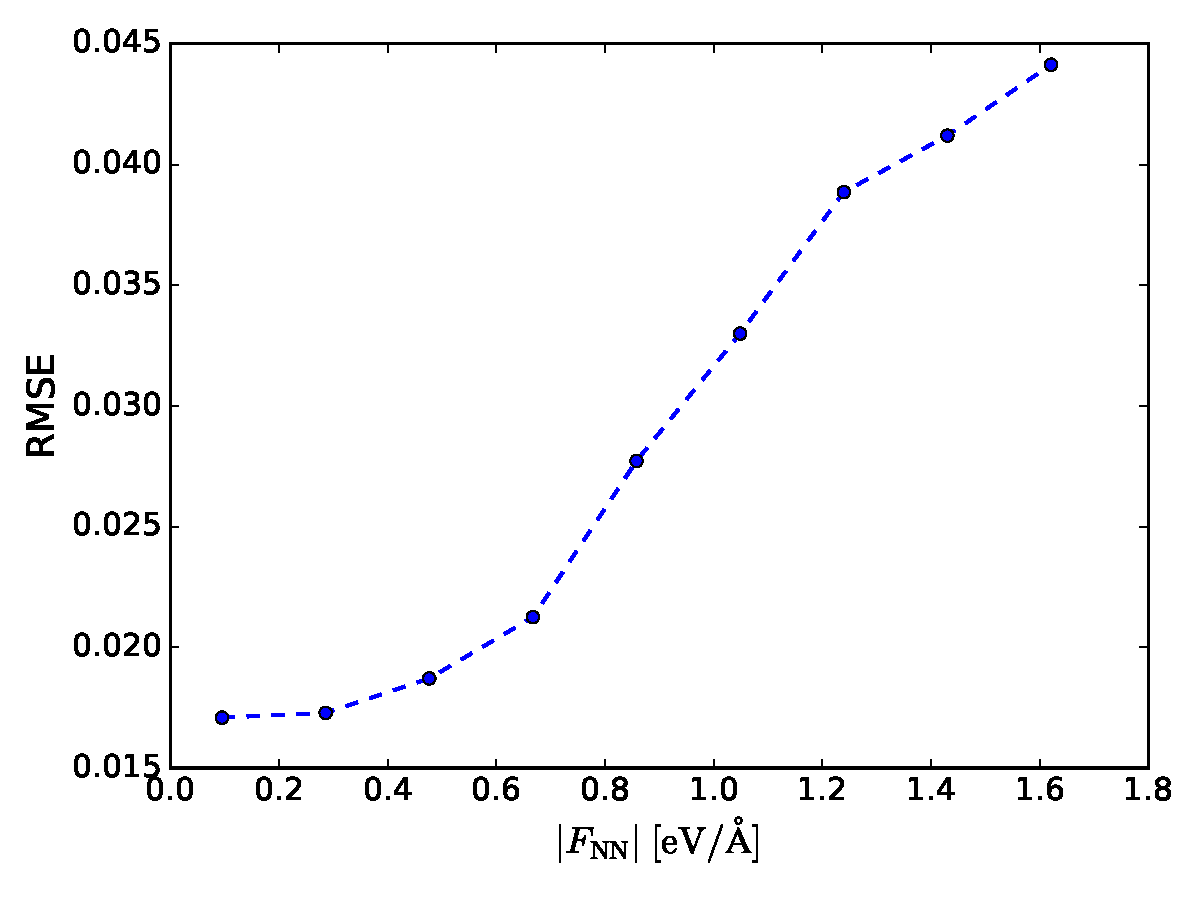
\includegraphics[width = 0.7\linewidth]{../Figures/Results/SiForces.pdf}
\end{block}

\end{frame}


\begin{frame}

\begin{block}{Radiell distribusjonsfunksjon $g(r)$}
 Sammenlikner tidsmidlet SW og NN.
 \centering
 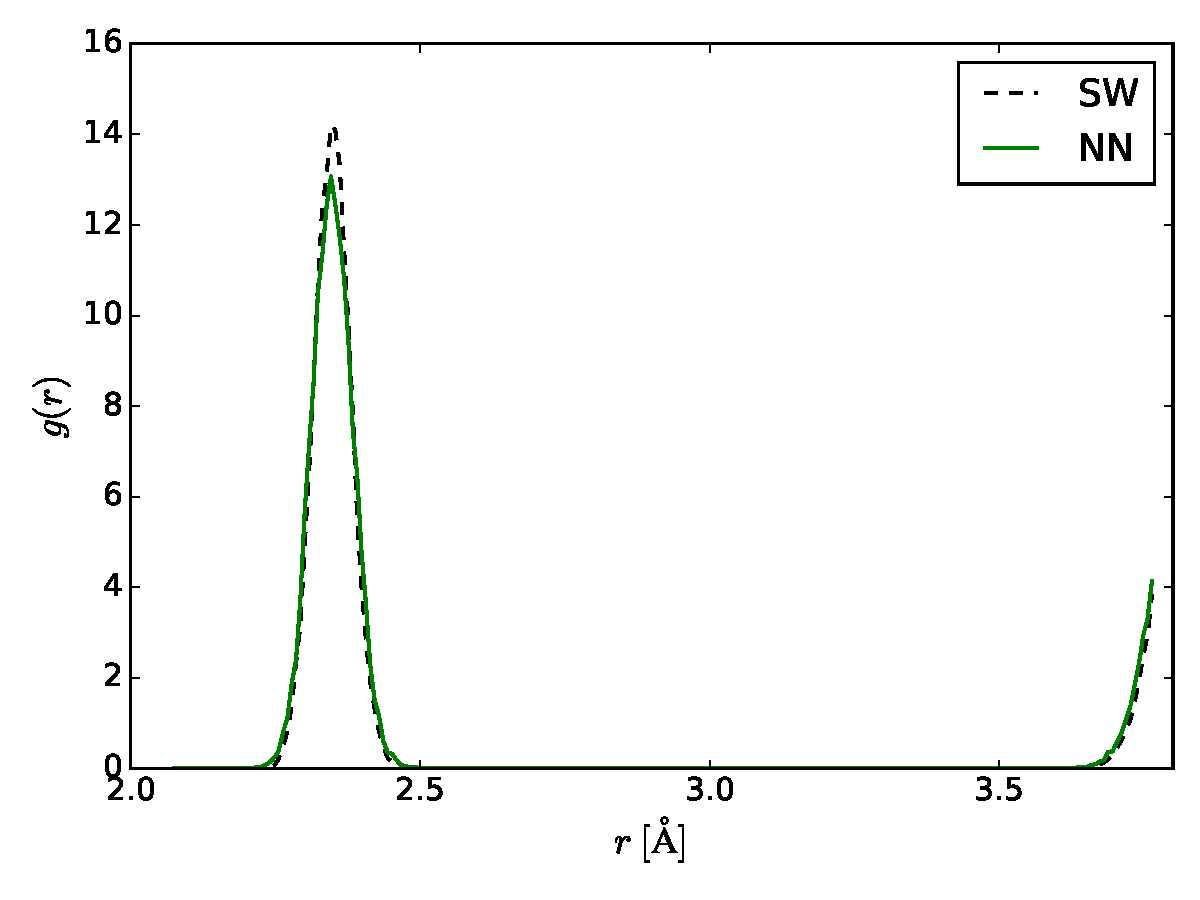
\includegraphics[width = 0.7\linewidth]{../Figures/Results/radialDist.pdf}
\end{block}

\end{frame}


\begin{frame}
 
\begin{block}{Mekaniske egenskaper}
 \begin{table}
 \centering
    \begin{tabular*}{10cm}{l @{\extracolsep{\fill}} lll}
      \toprule
      & NNP & Analytic SW & Relative error  \\ 
      \hline
      Bulk modulus    & 103.0  & 101.4 &  1.58 \% \\
      Shear modulus   & 53.6   & 56.4  &  5.22 \% \\
      Poisson ratio   & 0.348  & 0.335 &  3.88 \% \\
      \bottomrule
      \end{tabular*} 
 \end{table}
\end{block}

\end{frame}


\section{Konklusjon og fremtidig arbeid}


\begin{frame}

\begin{block}{Det ideelle potensial}
 \begin{itemize}
  \item Potensialet bør være nøyaktig.
        
  \item Burde finnes måter å systematisk forbedre potensialet.
        
  \item Potensialet bør være generelt og anvendbart på alle typer systemer.
	
  \item Potensialet bør kunne modellere faseoverganger.
	
  \item Potensialet bør være høydimensjonalt, dvs. avhenge av alle frihetsgrader.

 \end{itemize}
\end{block}

\end{frame}


\begin{frame}

\begin{block}{Det ideelle potensial fortsetter}
 \begin{itemize}
  \item Konstruksjonen av potensialet bør være så automatisert som mulig.
  \item Potensialet bør være prediktivt. 
  \item Potensialet bør være raskt å evaluere.
  \item Konstruksjonen bør ikke ta for mye tid. 
  \item Analytisk derivert bør være tilgjengelig. 
 \end{itemize}
\end{block}

\end{frame}


\begin{frame}

\begin{block}{Fremtidig arbeid}
 \begin{itemize}
  \item \textit{Ab inito} data. 
  \item Mer nøyaktige krefter. 
  \item Andre systemer. 
  \item Optimering. 
 \end{itemize}
\end{block}

\end{frame}






\end{document}
